%%%%%%%%%%%%%%%%%%%%%%%%%%%%%%%%%%%%%%%%%
% Journal Article
% LaTeX Template
% Version 1.2 (15/5/13)
%
% This template has been downloaded from:
% http://www.LaTeXTemplates.com
%
% Original author:
% Frits Wenneker (http://www.howtotex.com)
%
% License:
% CC BY-NC-SA 3.0 (http://creativecommons.org/licenses/by-nc-sa/3.0/)
%
%%%%%%%%%%%%%%%%%%%%%%%%%%%%%%%%%%%%%%%%%

%----------------------------------------------------------------------------------------
%	PACKAGES AND OTHER DOCUMENT CONFIGURATIONS
%----------------------------------------------------------------------------------------

\documentclass[twoside]{article}

\usepackage[utf8]{inputenc}
\usepackage[ngerman]{babel}

\usepackage[sc]{mathpazo} % Use the Palatino font
\usepackage[T1]{fontenc} % Use 8-bit encoding that has 256 glyphs
\linespread{1.05} % Line spacing - Palatino needs more space between lines
\usepackage{microtype} % Slightly tweak font spacing for aesthetics

\usepackage[hmarginratio=1:1,top=32mm,columnsep=20pt]{geometry} % Document margins
\usepackage{multicol} % Used for the two-column layout of the document
\usepackage[hang, small,labelfont=bf,up,textfont=it,up]{caption} % Custom captions under/above floats in tables or figures
\usepackage{booktabs} % Horizontal rules in tables
\usepackage{float} % Required for tables and figures in the multi-column environment - they need to be placed in specific locations with the [H] (e.g. \begin{table}[H])
\usepackage{hyperref} % For hyperlinks in the PDF
\hypersetup{%
  colorlinks   = true, %Colours links instead of ugly boxes
  breaklinks   = true,
  urlcolor     = blue, %Colour for external hyperlinks
  linkcolor    = blue, %Colour of internal links
  citecolor    = black %Colour of citations
}
\usepackage[vertfit]{breakurl}

\usepackage{lettrine} % The lettrine is the first enlarged letter at the beginning of the text
\usepackage{paralist} % Used for the compactitem environment which makes bullet points with less space between them

\usepackage{wasysym} 
\usepackage{marvosym}

\usepackage{apacite}

\usepackage{abstract} % Allows abstract customization
\renewcommand{\abstractnamefont}{\normalfont\bfseries} % Set the "Abstract" text to bold
\renewcommand{\abstracttextfont}{\normalfont\small\itshape} % Set the abstract itself to small italic text

\usepackage{titlesec} % Allows customization of titles
\renewcommand\thesection{\Roman{section}}
\titleformat{\section}[block]{\large\scshape\centering}{\thesection.}{1em}{} % Change the look of the section titles

\usepackage{graphicx}
\usepackage{pstricks}
\usepackage{pstricks-add}
\usepackage{pst-barcode}
\usepackage{pst-bar}
\usepackage{pst-plot}

\usepackage{fancyhdr} % Headers and footers
\pagestyle{fancy} % All pages have headers and footers
\fancyhead{} % Blank out the default header
\fancyfoot{} % Blank out the default footer
\fancyhead[C]{Scientifica Ambulo $\bullet$ Juni 2013 $\bullet$ Vol. I, No. 1} % Custom header text
\fancyfoot[RO,LE]{\thepage} % Custom footer text

\usepackage{cleveref}


%----------------------------------------------------------------------------------------
%	TITLE SECTION
%----------------------------------------------------------------------------------------

\title{\vspace{-15mm}\fontsize{24pt}{10pt}\selectfont\textbf{Die Ötschergräben}} % Article title

\author{%
Michael Fladischer
\and
Martina Schlaipfer
\and
Matthias Schlaipfer
\vspace{-5mm}
}
\date{}

%----------------------------------------------------------------------------------------

\begin{document}

\maketitle % Insert title

\thispagestyle{fancy} % All pages have headers and footers

%----------------------------------------------------------------------------------------
%	ABSTRACT
%----------------------------------------------------------------------------------------

\begin{abstract}

\noindent Vereinzelt auch als der ``Grand Canyon Österreichs'' bezeichnet, liegen die Ötschergräben
südlich am Fuße des Ötscher-Gebirgsmassivs. Der sechs Kilometer lange Graben wird vom Ötscherbach durchzogen,
der auf ener Höhe von ca. 1100 Meter über dem Meeresspiegel entspringt. Bekannt für sein klares Wasser und
die Wasserfälle, die entlang des Ötscherbaches in den Graben stürzen, sind die Ötschergräben ein beliebtes
Ausflugsziel für Wanderer.

\end{abstract}

%----------------------------------------------------------------------------------------
%	ARTICLE CONTENTS
%----------------------------------------------------------------------------------------

\begin{multicols}{2} % Two-column layout throughout the main article text

\section{Einleitung}

\lettrine[nindent=0em,lines=3]{D} as Ötscher-Gebirgsmassiv wird geologisch dem Alpenvorland als Teil der
Kalkalpen zugerechnet. Zusammen mit dem Schneeberg und dem Wiener Becken bildet es die Kalkvoralpen. \cite{SH:2012}

Das Ötschermassiv liegt im Gebiet des Naturparks Ötscher-Tormäuer, welcher 1970 als Folge einer Protestbewegung gegen ein neues Wasserkraftwerk an der Erlauf
entstand \cite{NOT:2013:Online}. Das Gebiet um den Naturpark ist vor allem seit der Zuwanderung eines Bärenmännchens aus Slowenien Anfang der 1970er Jahre und
der darauf folgenden Ansiedelung von drei weiteren Bären in den nördlichen Kalkalpen bekannt.

Im Sommer des Jahres 2012 unternahmen kälteresistente Mitglieder der bergbegeisterten Familie Maierhofer gleich zwei Wanderungen, welche auch ein Bad in den
Bächen abseits der Wanderwege einschloß. Dies waren zuerst in der Bärenschützklamm und dann, im größeren Rahmen, in den Ötschergräben, nahe den Mirafällen.

\begin{figure}[H]
\begin{center}
  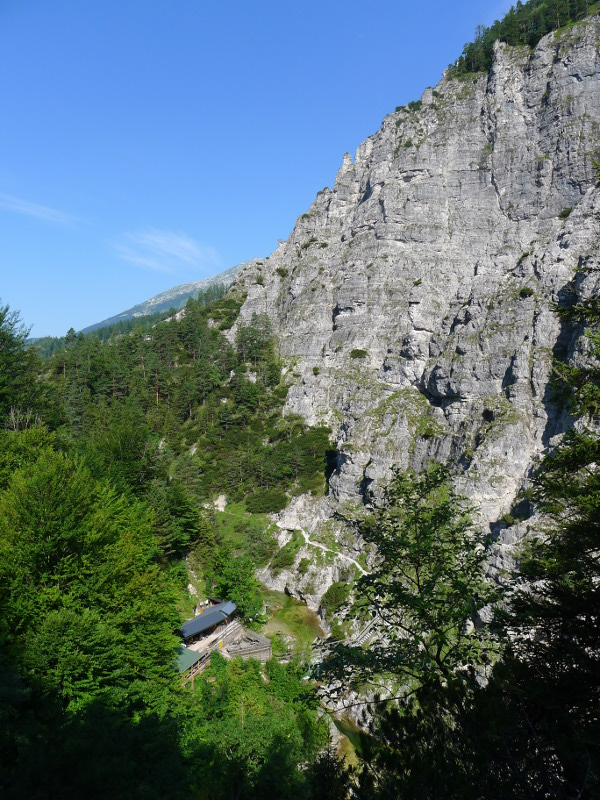
\includegraphics[natwidth=600, natheight=800, width=.45\textwidth]{Figures/oetschergraeben.jpg}
\end{center}
\caption{Schööön!}
\label{fig:oetschergraeben}
\end{figure}
% I forgot how to bar chart :-)
    %\psset{unit=0.4in}%
    %\begin{pspicture}(0,-0.5)(4,11)%
        %\psgrid
        %\readpsbardata{\data}{feedback.csv}%
        %\psgrid[xunit=1.5in,gridlabels=0,%
            %subgriddiv=0,griddots=20](0,0)(1,11)%
        %\psaxes[axesstyle=frame,Ox=0,Dx=1,labels=y,%
            %ticks=y](0,0)(2,11)%
        %\psbarchart[
            %barstyle={red,blue}
        %]{\data}%
    %\end{pspicture}
    %\caption{Rückmeldungen zu Bärenschützklamm und Ötschergräben 2012}
    %\label{fig:feedback}
%\begin{figure}
%\resizebox{\columnwidth}{!}{
%\begin{pspicture}(-2.1,-2.1)(2.1,2.1)
%\degrees[100]
%\pswedge[fillstyle=solid,fillcolor=gray,hatchcolor=gray]{2}{0}{17 }
%\rput(1.2; 8 ){\psframebox*{\small 17 \%}}
%\uput{2.2}[ 8 ](0;0){\Large A él}
%\pswedge[fillstyle=hlines,fillcolor=gray,hatchcolor=gray]{2}{17 }{42 }
%\rput(1.2;29 ){\psframebox*{\Large 25 \%}}
%\uput{2.2}[29 ](0;0){\Large A dém}
%\pswedge[fillstyle=solid,fillcolor=white,hatchcolor=white]{2}{42 }{58 }
%\rput(1.2;50 ){\psframebox*{\Large 17 \%}}
%\uput{2.2}[50 ](0;0){\Large égal}
%\pswedge[fillstyle=hlines,fillcolor=gray,hatchcolor=gray]{2}{58 }{83 }
%\rput(1.2;71 ){\psframebox*{\Large 25 \%}}
%\uput{2.2}[71 ](0;0){\Large B dém}
%\pswedge[fillstyle=solid,fillcolor=gray,hatchcolor=gray]{2}{83 }{100 }
%\rput(1.2;92 ){\psframebox*{\Large 17 \%}}
%\uput{2.2}[92 ](0;0){\Large B él}
%\rput(0;0){\psframebox*{\bfseries 0/0}}
%\end{pspicture}
%}
%\end{figure}

Aufgrund des Begeisterung einer representativen Population der Teilnehmer aus dem Jahr 2012 soll auch heuer wieder eine Wanderung in das Gebiet der
Ötschergräben unter möglichst umfassender Teilnahme aller Familienmitglieder stattfinden.

%------------------------------------------------

\section{Ablauf}

\begin{itemize}
    \item Wo treffen wir uns?
    \item Wo geht es hin?
    \item Welche Zwischenstopps gibt es?
    \item Wann kommen wird in etwa zu den Mirafällen?
    \item Kehren wir beim Ötscherhias ein?
    \item Wann geht es zurück zu den Autos?
    \item Benutzen wir die Mariazellerbahn?
\end{itemize}


%------------------------------------------------

\section{Ausrüstung}

\lettrine[nindent=0em,lines=3]{E} ine Wanderung, welche mit einem Bad im Gebirgsbach oder in der Gumpe eines Wasserfalls kombiniert wird, macht es erforderlich,
ein Mindestmaß an empfohlener Ausrüstung mitzuführen.

\begin{itemize}
    \item Badebekleidung (unter der Wanderkleidung oder separat).
    \item Trockene Unterwäsche zum Wechseln.
    \item Ein Badetuch.
    \item Sonnencreme, auch während der Wanderung zu benutzen.
    \item Badeschlapfen (optional).
\end{itemize}

\begin{figure}[H]
\begin{center}
  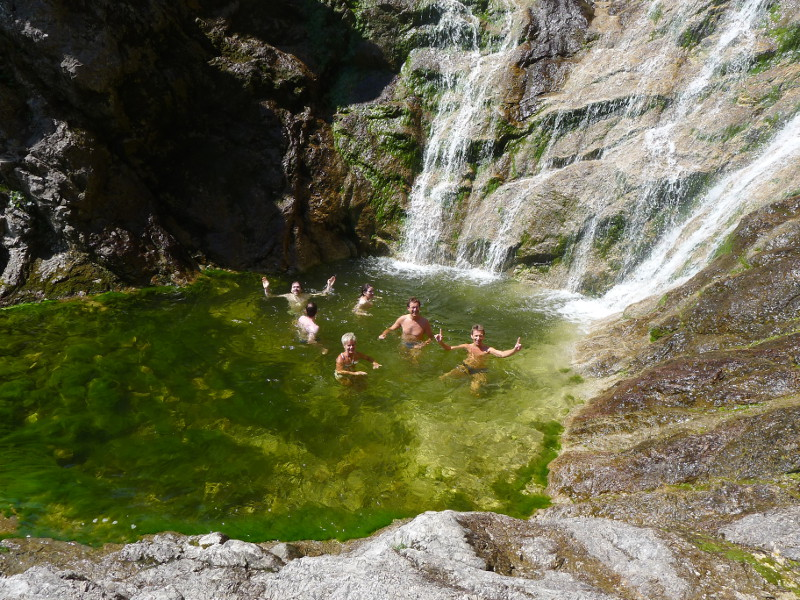
\includegraphics[natwidth=800, natheight=600, width=.45\textwidth]{Figures/bad.jpg}
\end{center}
\caption{Erfrischend!}
\label{fig:bad}
\end{figure}

%------------------------------------------------

\section{Teilnahme}

\lettrine[nindent=0em,lines=3]{D} ie Abstimmung des Termins erfolgt über einen \href{http://www.doodle.com/m6ywebgyvg6632ig}{Doodle}. Smartphone-Benutzer
können den QR-code scannen um auf die entsprechende Seite zu gelangen. Für Benutzer von handelsüblichen PDF-Readern genügt ein Klick auf das blau hervorgehobene
Wort.

%\href{http://www.doodle.com/m6ywebgyvg6632ig}{%
%\pspicture(\columnwidth,\columnwidth)
%\psbarcode{http://www.doodle.com/m6ywebgyvg6632ig}{height=2.4 width=2.4}{qrcode}
%\endpspicture
%}

Es stehen fünf Termine mit je drei Uhrzeiten zu Auswahl, wobei die Uhrzeit festlegt, wann wir uns am Parkplatz in Wienerbruck/Erlaufklause treffen.

%------------------------------------------------

\section{Rückfragen}

\lettrine[nindent=0em,lines=3]{B} ei allfälligen Rückfragen stehen die Autoren selbstverständlich zur Verfügung. Es können auch Kommentare im Doodle
 hinterlassen werden. Sollte es passieren, dass nach der Zusage zu einem Termin dieser doch nicht wahrgenommen werden kann, so bitten wir um kurze Mitteilung.

\begin{tabular}{l l}
\Letter \ \href{mailto:michael@fladi.at}{Michael Fladischer} & \phone \ 0660/4806299 \\
\Letter \ \href{mailto:mschlaipfer@gmx.net}{Martina Schlaipfer} & \phone \ 0680/1302672 \\
\Letter \ \href{mailto:m.schlaipfer@gmail.com}{Matthias Schlaipfer} & \phone \ 0680/2333950 \\
\end{tabular}


%----------------------------------------------------------------------------------------
%	REFERENCE LIST
%----------------------------------------------------------------------------------------

\bibliographystyle{apacite}
\bibliography{literature}

%----------------------------------------------------------------------------------------

\end{multicols}

\end{document}
